\subsection{Gaussian mixtures}

\begin{frame}{Gaussian mixture model (Old Faithful data set)}
  \vspace{-15pt}
  \begin{figure}
    \centering
    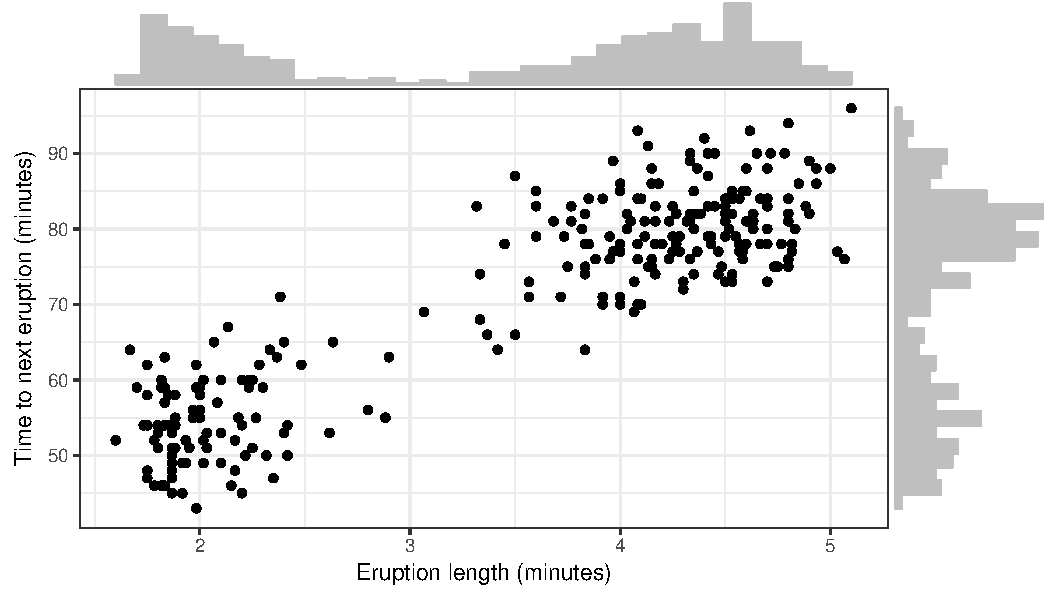
\includegraphics[scale=0.65]{figure/faithful_scatter}
  \end{figure}
  \vspace{-13pt}
  \begin{itemize}
    \item Let $\bx_i \in \bbR^d$ and assume $\bx_i \iid \sum_{k=1}^K \pi_{k} \N_d(\bmu_k,\bPsi_k^{-1})$ for $i=1,\dots,n$.
  \end{itemize}
\end{frame}

\begin{frame}{Gaussian mixture model}  
  \vspace{-4.5mm}
  \onslide<2->{
  \begin{tikzpicture}[scale=1.1, transform shape]
    \tikzstyle{main}=[circle, minimum size = 10mm, thick, draw =black!80, node distance = 16mm]
    \tikzstyle{connect}=[-latex, thick]
    \tikzstyle{box}=[rectangle, draw=black!100]
    \node[main] (pi) {$\bpi$};
    \only<3->{\node[main,draw=colred] (pi) {\color{colred} $\bpi$};}
    \node[main] (z) [right=of pi,xshift=-0.65cm] {$\bz_i$};  %fill=black!10, double, double distance=0.6mm
    \node[main] (x) [right=of z,xshift=-0.5cm] {$\bx_i$};
    \node[main] (mu) [above=of z,yshift=-0.7cm] {$\bmu_k$};  
    \only<3->{\node[main,draw=colblu] (mu) [above=of z,yshift=-0.7cm] {\color{colblu} $\bmu_k$};}
    \node[main] (Psi) [above=of x,yshift=-0.7cm] {$\bPsi_k$};  
    \only<3->{\node[main,draw=colgre] (Psi) [above=of x,yshift=-0.7cm] {\color{colgre} $\bPsi_k$};}
    \path (pi)  edge [connect] (z)
          (z)   edge [connect] (x)
  		  (Psi) edge [connect] (mu) 
   		  (mu)  edge [connect] (x)
   		  (Psi) edge [connect] (x);
    \node[rectangle, draw=black!100, fit= {(mu) ($(Psi.north east) + (0,0.5cm)$)}] {}; 
    \node[rectangle, fit=(mu) (Psi), yshift=6.8mm, xshift=6.5mm] {\small$k=1,\dots,K$}; 
    \node[rectangle, draw=black!100, fit={(z) ($(x.south east) + (0,-0.5cm)$)}] {}; 
    \node[rectangle, fit=(z) (x), yshift=-9.9mm, xshift=7.5mm] {\small $i=1,\dots,n$}; 
  \end{tikzpicture}
  }

  \onslide<3->{  
  \begin{textblock*}{0.47\textwidth}(0.55\textwidth,1.2cm)
    \begin{block}{}
    \vspace{-1.6em}
      \begin{align*}
        &p(\bx,\bz,\bpi,\bmu,\bPsi) \\
        &= p(\bx|\bz,\bmu,\bPsi)p(\bz|\bpi) \\
        &\phantom{ = } \ \times p(\bpi)p(\bmu|\bPsi)p(\bPsi) \\
        &= p(\bx|\bz,\bmu,\bPsi)p(\bz|\bpi) \\
        &\phantom{ = } \ \times {\color{colred} \Dir_K(\bpi|\alpha_{01},\dots,\alpha_{0K})} \\
        &\phantom{ = } \ \times {\color{colblu} {\textstyle\prod}_{k=1}^K \N_d(\bmu_k| \bmm_0, \big(\kappa_0\bPsi_k)^{-1}\big)} \\
        &\phantom{ = } \ \times {\color{colgre} {\textstyle\prod}_{k=1}^K \Wis_d(\bPsi_k| \bW_0,\nu_0\big)}      
      \end{align*}
    \end{block}
  \end{textblock*}
  }

  \vspace{-2.5mm}
  \begin{itemize}
    \item Introduce $\bz_i = (z_{i1},\dots,z_{iK})$, a $1$-of-$K$ binary vector, where each $z_{ik} \sim \Bern(\pi_k)$.
    \item Assuming $\bz = \{\bz_1,\dots,\bz_n \}$ are observed along with $\bx = \{\bx_1,\dots,\bx_n \}$,
    \[
      p(\bx|\bz,\bmu,\bPsi) = \prod_{i=1}^n \prod_{k=1}^K \N_d(\bx_i|\bmu_k,\bPsi_k^{-1})^{z_{ik}}.
    \]
  \end{itemize}
\end{frame}

\begin{frame}[label=vigmm]{Variational inference for GMM}
  \begin{itemize}
    \item Assume the mean-field posterior density
    \begin{align*}
      q(\bz,\bpi,\bmu,\bPsi) &= q(\bz)q(\bpi,\bmu,\bPsi) \\
      &= q(\bz)q(\bpi)q(\bmu|\bPsi)q(\bPsi).
    \end{align*}
  \end{itemize}
  
  \begin{center}
    \scalebox{0.9}{
    \begin{minipage}{\linewidth}
  \begin{algorithm}[H]
    \caption{CAVI for GMM}\label{alg:gmm}
    \begin{algorithmic}[1]
      \State \textbf{initialise} Variational factors $q(\bz)$, $q(\bpi)$ and $q(\bmu,\bPsi)$
      \While{$\cL(q)$ not converged}
        \State $q(z_{ik}) \gets \Bern(\cdot)$
        \State $q(\bpi) \gets \Dir_K(\cdot)$
        \State $q(\bmu|\bPsi) \gets \N_d(\cdot,\cdot)$
        \State $q(\bPsi) \gets \Wis_d(\cdot,\cdot)$
        \State $\cL(q) \gets \E_{ q}[\log p(\bx,\bz,\bpi,\bmu,\bPsi)] - \E_{ q}[\log q(\bz,\bpi,\bmu,\bPsi)]$
      \EndWhile
      \State \textbf{return} $\tilde q(\bz,\bpi,\bmu,\bPsi) = \tilde q(\bz) \tilde q(\bpi) \tilde q(\bmu|\bPsi) \tilde q(\bPsi)$ 
    \end{algorithmic}
  \end{algorithm}
      \end{minipage}%
    }
  \end{center}
  
  \begin{textblock*}{3cm}(.9\textwidth,0.498\textheight)%
    \hyperlink{vigmmsoln}{\beamerbutton{details}}      
  \end{textblock*}
\end{frame}

\begin{frame}{Variational inference for GMM (cont.)}
  \vspace{-6pt}
  \begin{figure}
    \centering\hspace{-10pt}
    \only<1|handout:1>{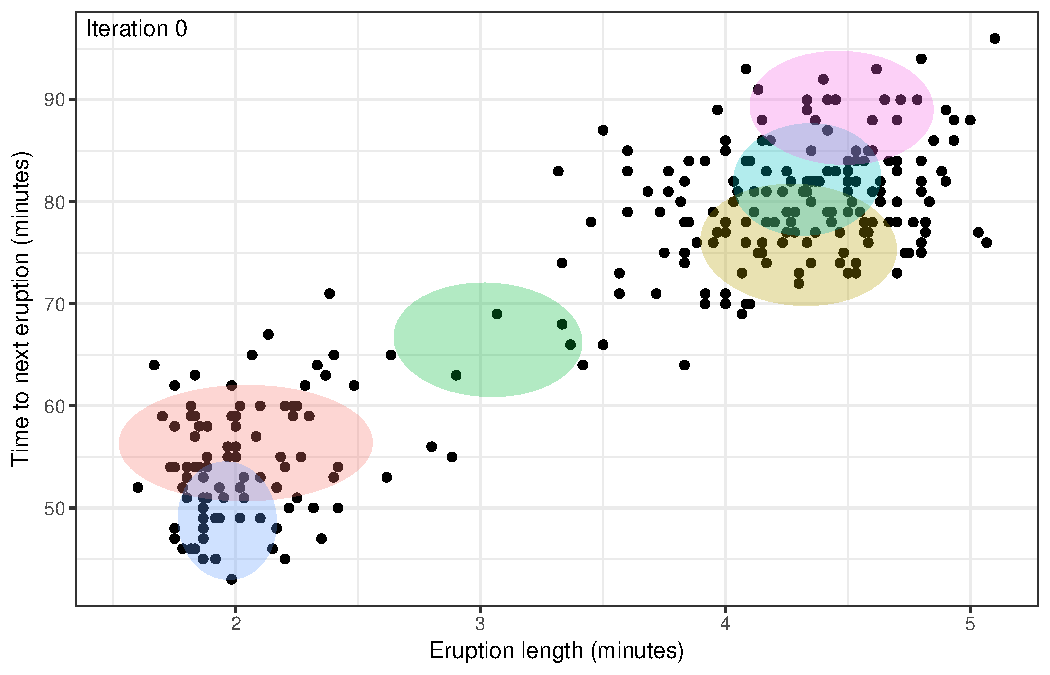
\includegraphics[scale=0.67]{figure/faithful_iter_1}}
    \only<2|handout:2>{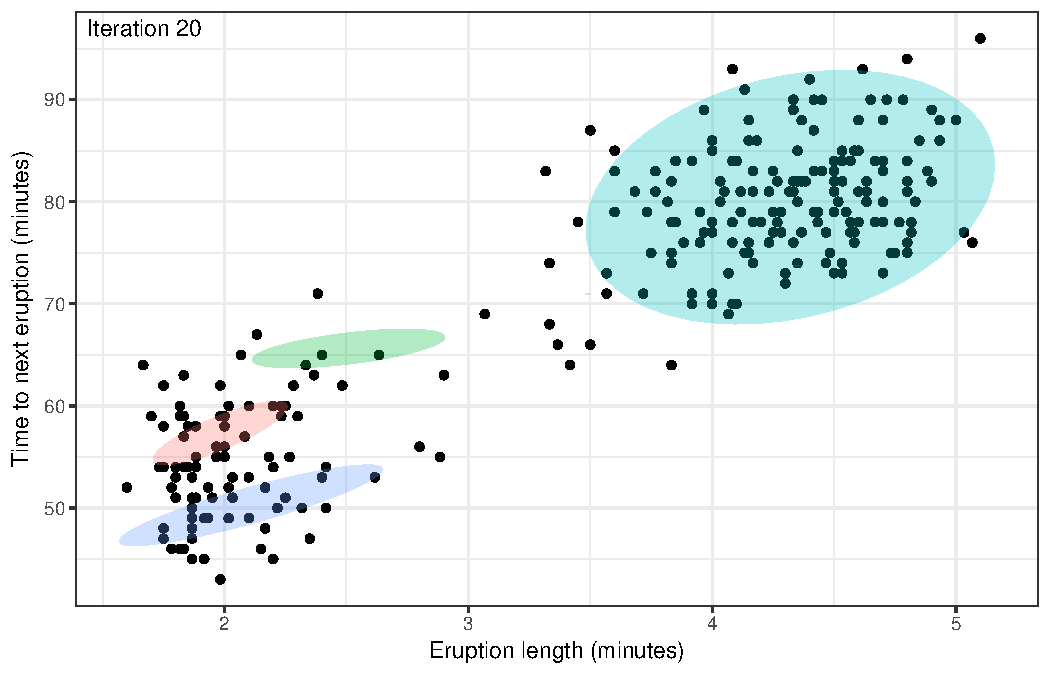
\includegraphics[scale=0.67]{figure/faithful_iter_2}}
    \only<3|handout:0>{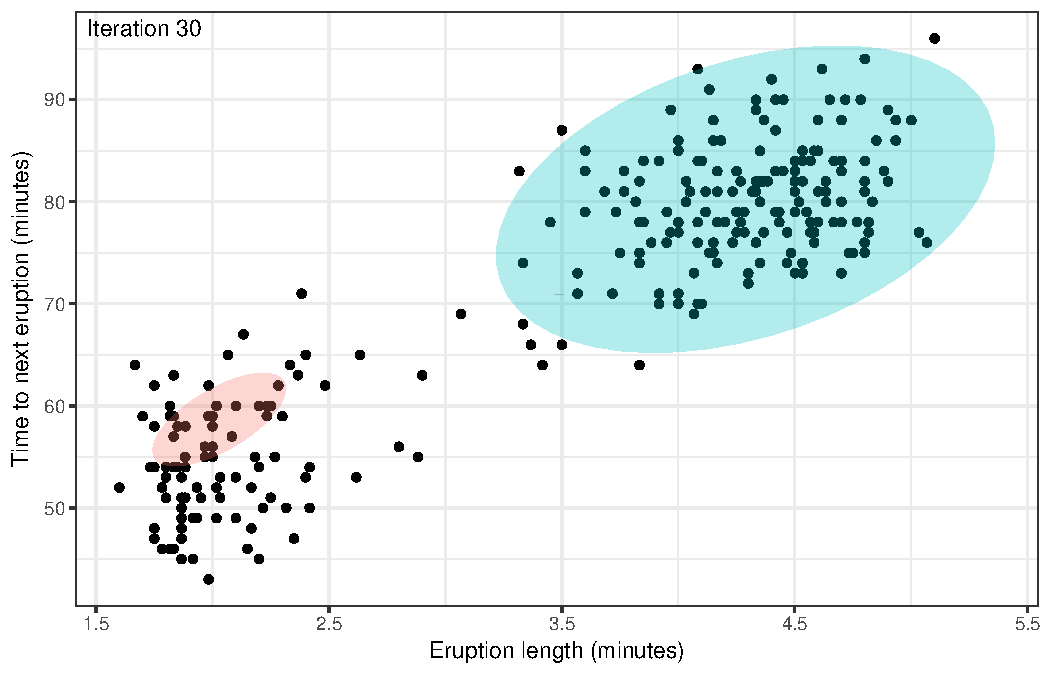
\includegraphics[scale=0.67]{figure/faithful_iter_3}}
    \only<4|handout:3>{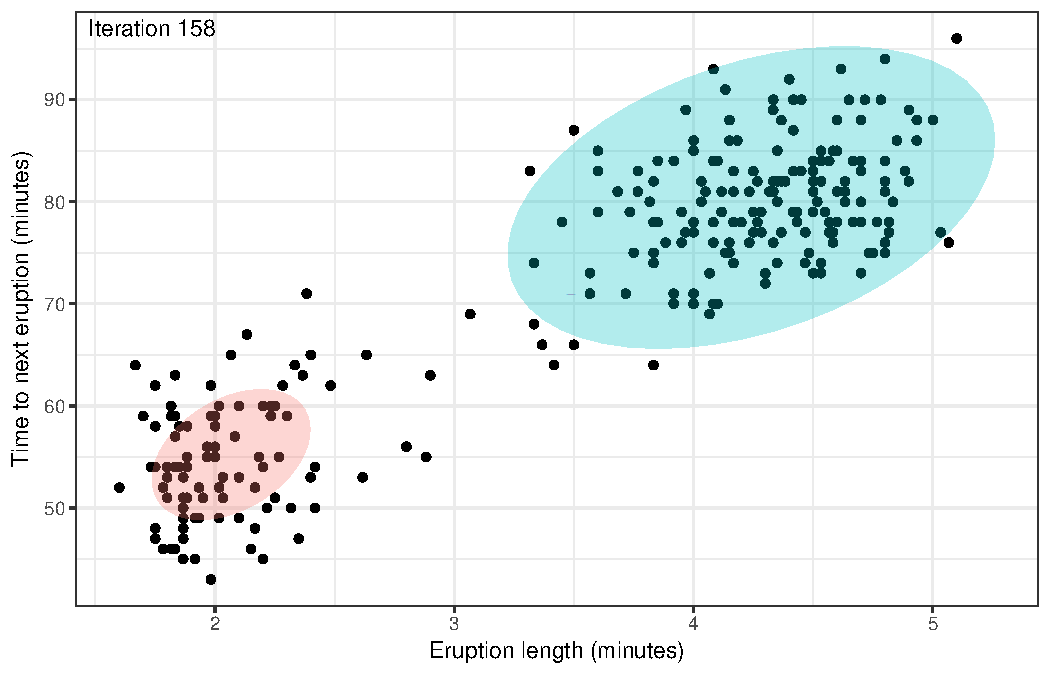
\includegraphics[scale=0.67]{figure/faithful_iter_4}}
  \end{figure}
\end{frame}

\begin{frame}{Final thoughts on variational GMM}
  \begin{itemize}
    \item Similar algorithm to the EM, and therefore similar computational time.
    \item Can extend to mixture of bernoullis a.k.a. latent class analysis. 
    \item \textbf{PROS}:
    \begin{itemize}
      \item Automatic selection of number of mixture components.
      \item Less pathological special cases compared to EM solutions because regularised by prior information.
      \item Less sensitive to number of parameters/components.
    \end{itemize}
    \item \textbf{CONS}:
    \begin{itemize}
      \item Hyperparameter tuning.
    \end{itemize}
  \end{itemize}
\end{frame}
